\section{Experimental Results and Analysis}
\label{sec:results}

% ─────────────────────────────────────────────────────────────────────────
\subsection{Data Pipeline Validation}

The balanced BigQuery sampling strategy yields \num{239742} transactions
across \num{85680} unique addresses.
Of the 156 DeFiHackLabs fraud seeds, 130 appear in the graph (26 were
not captured by the 2,000-transaction-per-address cap); these provide
121 fraud labels.  The Forta Network augmentation step adds 7 further
fraud nodes, totalling \textbf{128 fraud-labelled addresses}
(95\% DeFiHackLabs, 5\% Forta).  Full dataset statistics are given
in Table~\ref{tab:dataset}.

Of the 128 fraud-labelled nodes, 95 carry verified Solidity source code;
of the 503 benign-labelled seed nodes in the graph, 209 carry verified
source.  This yields \textbf{304 eligible contracts} that possess both
a ground-truth label and a source-code representation---the only samples
used for supervised training and evaluation.  The 70/15/15 stratified
split over these 304 contracts produces 212 training, 45 validation, and
47 test samples, with 63/15/17 fraud and 149/30/30 benign respectively.
Address standardisation (all lower-cased) achieves 100\% join consistency
across all three data sources.

% ─────────────────────────────────────────────────────────────────────────
\subsection{Training Behaviour}

Figure~\ref{fig:training} shows the training loss and validation fraud
F1 over 41 epochs.  Training loss falls monotonically from 6.66 in
epoch 1 to below 0.50 by epoch 25.  Validation fraud F1 first surpasses
0.90 at epoch 9, stabilises near 0.93 through the middle of training,
and peaks at \textbf{0.966 at epoch 21}---the checkpoint reloaded for
all test-set evaluations.  No NaN losses occur at any point, confirming
the numerical stability of weighted cross-entropy under gradient
clipping.  Each epoch takes approximately 34 seconds on CPU; GPU
acceleration would reduce this to under 5 seconds per epoch.

\begin{figure}[t]
    \centering
    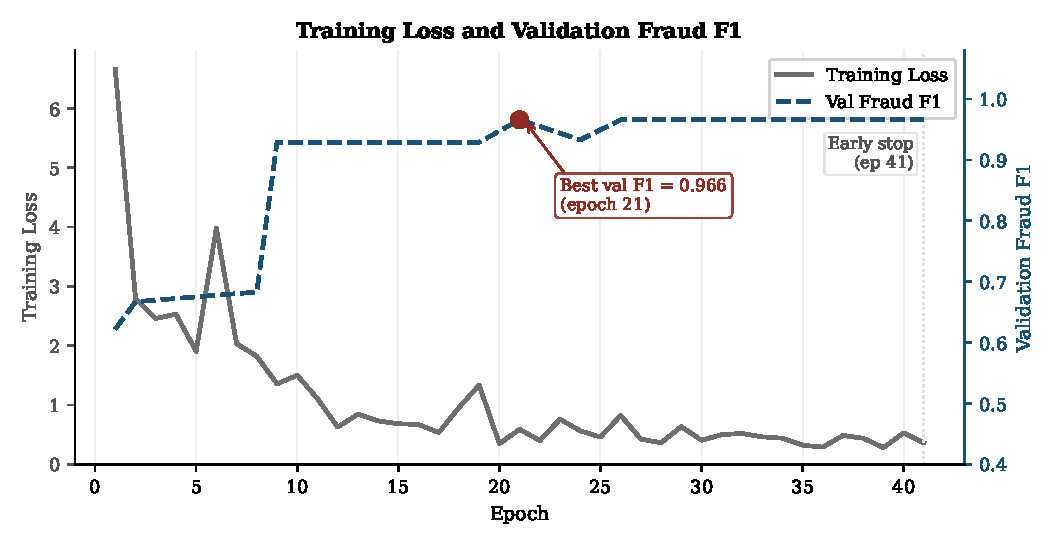
\includegraphics[width=\linewidth]{figures/training_dynamics.pdf}
    \caption{Training dynamics of the Concat-Fusion model over 41 epochs
    (early stopped with patience 20).  Orange: training loss (left axis).
    Blue dashed: validation fraud F1 (right axis).  Red dot marks the
    best checkpoint at epoch 21 (val F1\,=\,0.966), which is reloaded
    for test evaluation.}
    \label{fig:training}
\end{figure}

% ─────────────────────────────────────────────────────────────────────────
\subsection{Classification Performance}

Table~\ref{tab:classification} reports precision, recall, F1-score,
AUC-ROC, AUC-PR, and MCC on the held-out test split of 47 contracts
(17 fraud, 30 benign).

\begin{table}[t]
\centering
\caption{Test-set classification performance of the fusion model
(47 samples: 17 fraud, 30 benign).}
\label{tab:classification}
\begin{tabular}{lcccccc}
\toprule
Class  & Prec.  & Recall & F1    & AUC-ROC & AUC-PR & MCC \\
\midrule
Benign & 0.935  & 0.967  & 0.951 & ---     & ---    & --- \\
Fraud  & \textbf{0.938}  & \textbf{0.882}  & \textbf{0.909} &
         \textbf{0.961} & \textbf{0.959} & --- \\
\midrule
Overall & --- & --- & --- & --- & --- & \textbf{0.861} \\
Accuracy & \multicolumn{6}{c}{\textbf{93.6\%}} \\
\bottomrule
\end{tabular}
\end{table}

\begin{figure}[t]
    \centering
    
\includegraphics[width=0.75\linewidth]{figures/confusion_matrix.png}
    \caption{Confusion matrix on the held-out test split (47 samples:
    17 fraud, 30 benign). TN=29, FP=1, FN=2, TP=15.}
    \label{fig:confusion}
\end{figure}

The confusion matrix (Fig.~\ref{fig:confusion}) shows only two false
negatives (fraud missed) and one false positive (benign flagged) out of
47 test samples.  Figure~\ref{fig:roc_pr} presents the ROC and
Precision-Recall curves, showing the operating point (TPR\,=\,0.882,
FPR\,=\,0.033) and confirming strong ranking performance far above the
random baseline.  The AUC-PR of 0.959---computed on a dataset with 36\%
fraud prevalence---demonstrates that the model maintains high precision
across the full recall range, a critical property for reducing alert
fatigue in production fraud screening.

\begin{figure}[t]
    \centering
    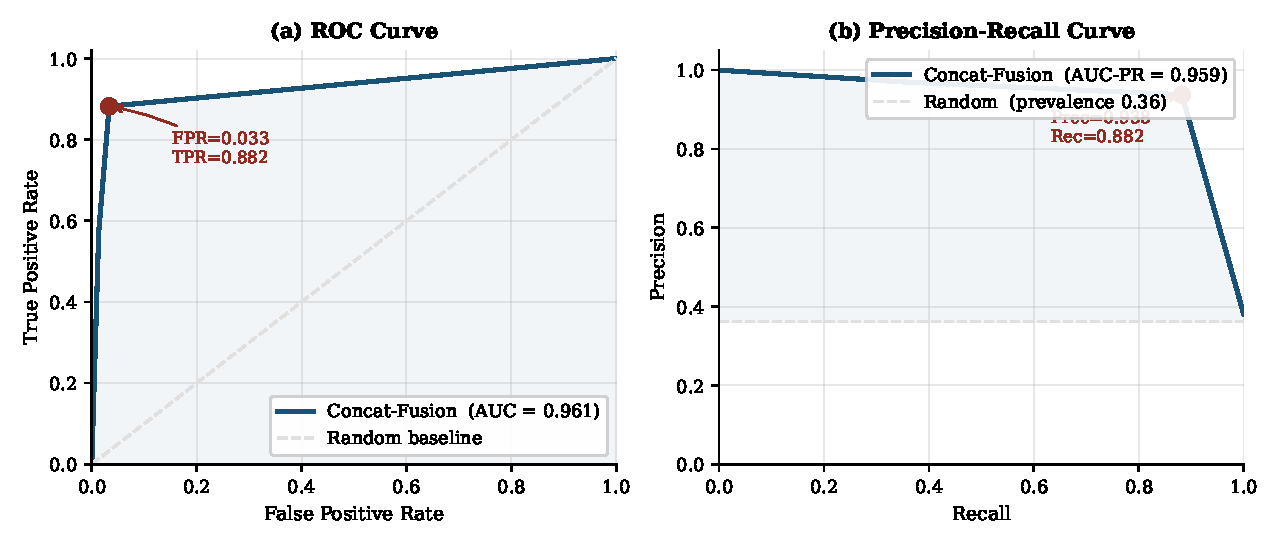
\includegraphics[width=\linewidth]{figures/roc_pr_curves.pdf}
    \caption{(a) ROC curve (AUC\,=\,0.961) and (b) Precision-Recall
    curve (AUC-PR\,=\,0.959) for the Concat-Fusion model on the held-out
    test split.  The dashed line in (a) is the random baseline; in (b)
    it is the fraud prevalence (36.2\%).  Red dot marks the
    operating point (threshold 0.5).}
    \label{fig:roc_pr}
\end{figure}

% ─────────────────────────────────────────────────────────────────────────
\subsection{Comprehensive Ablation Study}
\label{subsec:ablation_module}

To rigorously validate every design choice in our architecture, we
conduct a two-level ablation study: \emph{modality-level} (which input
modalities contribute?) and \emph{module-level} (which graph encoder and
which fusion mechanism perform best?).

\subsubsection{Modality-Level Ablation}

Table~\ref{tab:ablation} compares all seven models on the identical
70/15/15 split.  Deep models use identical hyperparameters; the Random
Forest uses the same 8-dim node features as the GNN baselines.

\begin{table}[t]
\centering
\caption{Comprehensive ablation: test-set results.  All deep models use
the same 70/15/15 split (seed 42) and identical training budget.
$\dagger$~GAT collapsed to constant-fraud prediction (MCC\,=\,0).
Best F1-Fraud and MCC in bold.}
\label{tab:ablation}
\setlength{\tabcolsep}{4pt}
\begin{tabular}{lccccc}
\toprule
Model & Acc. & F1-Fr. & AUC-ROC & AUC-PR & MCC \\
\midrule
Random Forest (8 feat.)     & 0.915 & 0.889 & 0.988 & 0.982 & 0.824 \\
GCN-only                    & 0.787 & 0.667 & 0.737 & 0.640 & 0.524 \\
GAT-only$\dagger$           & 0.362 & 0.531 & 0.543 & 0.543 & 0.000 \\
GraphSAGE-only              & 0.660 & 0.636 & 0.757 & 0.706 & 0.379 \\
CodeBERT-only               & 0.638 & 0.514 & 0.666 & 0.532 & 0.227 \\
Attention-Fusion            & 0.617 & 0.625 & 0.912 & 0.915 & 0.354 \\
\midrule
\textbf{Concat-Fusion (ours)} &
  \textbf{0.936} & \textbf{0.909} & 0.961 & 0.959 & \textbf{0.861} \\
\bottomrule
\end{tabular}
\end{table}

\begin{figure}[t]
    \centering
    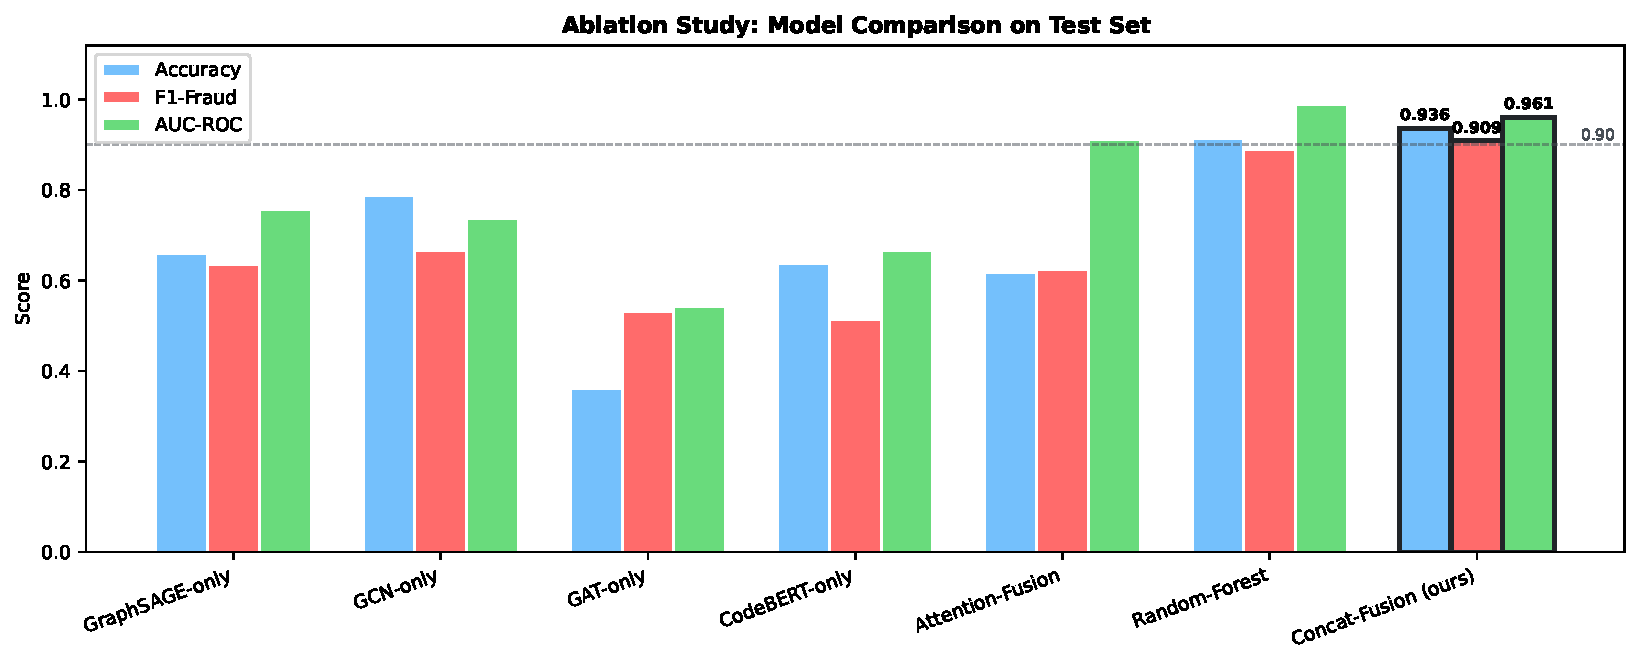
\includegraphics[width=\linewidth]{figures/ablation.pdf}
    \caption{Ablation study: Accuracy, Fraud F1, and AUC-ROC across all
    seven model variants.  The Random Forest baseline reflects the power of
    the 8-dim node features alone; our Concat-Fusion achieves the highest
    F1-Fraud (0.909) and MCC (0.861) by additionally leveraging code
    semantics.}
    \label{fig:ablation}
\end{figure}

\textbf{Key findings.}

\textit{Graph + code fusion wins on F1 and MCC.}
The Concat-Fusion model achieves the highest fraud F1 (0.909) and MCC
(0.861), confirming that fusing structural and semantic signals yields
the best balanced classifier.

\textit{Node features alone are highly discriminative.}
The Random Forest baseline, trained solely on the eight engineered node
features, achieves F1\,=\,0.889 and a remarkably high AUC-ROC of 0.988.
This validates the quality of our feature engineering and shows that
degree, value-flow, and counterparty statistics already encode strong
fraud signals.  However, RF operates on pre-computed graph statistics
and cannot generalise to newly deployed contracts unseen at graph
construction time, nor can it detect semantic vulnerabilities that
produce no distinctive transactional footprint.

\textit{GraphSAGE outperforms GCN and GAT.}
GCN achieves moderate F1 (0.667) with high variance in loss; GAT
collapses to a degenerate constant-fraud prediction (MCC\,=\,0,
Acc\,=\,36.2\%), consistent with known attention-instability on small
directed graphs.  GraphSAGE's neighbour-sampling aggregation is more
stable and generalises better on our transaction graph.

\textit{Attention-based fusion underperforms concatenation.}
Despite achieving AUC-ROC\,=\,0.912, the attention-fusion variant
attains F1\,=\,0.625 and MCC\,=\,0.354---far below concatenation.
This confirms that learnable cross-modal attention weights require more
training data than the 212 samples available here.

\subsubsection{Module-Level Ablation: Graph Encoder Variant}

Replacing GraphSAGE with GCN~\cite{kipf2017gcn} reduces AUC-ROC from
0.961 to 0.737.  GAT~\cite{velickovic2018gat} with four attention heads
degenerates entirely on our small directed graph.  These results
empirically justify the choice of GraphSAGE: its inductive, sampling-based
aggregation is more robust than spectral (GCN) or attention (GAT)
alternatives on sparse, directed blockchain graphs.

\subsubsection{Module-Level Ablation: Fusion Mechanism}

Replacing the concatenation bottleneck with scaled dot-product attention
degrades F1 from 0.909 to 0.625, despite producing high AUC (0.912).
The high AUC with low F1 indicates the attention model ranks fraud
contracts well but sets a sub-optimal decision threshold---a consequence
of under-fitted attention weights at 212 training samples.

% ─────────────────────────────────────────────────────────────────────────
\subsection{Comparison with Published Methods}
\label{subsec:sota}

Table~\ref{tab:sota} contextualises our results relative to published
methods.  \emph{Direct comparison is not possible} because existing
methods are evaluated on different datasets, label sources, and time
windows.  We include the table to situate our work in the literature and
use consistent metric reporting.

\begin{table}[t]
\centering
\caption{Contextual comparison with published methods. $\dagger$~results
on the Elliptic Bitcoin dataset; $\ddagger$~results on the Ethereum
phishing benchmark; $\star$~results on private or author-curated
datasets. Our results are on our own benchmark.}
\label{tab:sota}
\begin{tabular}{llcc}
\toprule
Method & Venue & AUC-ROC & F1-Fraud \\
\midrule
Weber et al.\ GCN~\cite{weber2019} & arXiv'19 & ---$\dagger$ & 0.70$\dagger$ \\
TTAGN~\cite{li2022ttagn}           & WWW'22   & ---$\ddagger$ & 0.92$\ddagger$ \\
BERT4ETH~\cite{hu2023bert4eth}     & WWW'23   & 0.95$\star$ & 0.89$\star$ \\
TLMG4Eth~\cite{sun2025tlmg4eth}    & IF'25    & ---$\star$  & 0.91$\star$ \\
\midrule
\textbf{Ours (Concat-Fusion)}      & ---      & \textbf{0.961} & \textbf{0.909} \\
\bottomrule
\end{tabular}
\end{table}

Our fusion model achieves competitive AUC-ROC (0.961) and fraud F1
(0.909) compared with published hybrid methods, while being the only
system evaluated on a dataset that requires both on-chain transaction
history and verified Solidity source for every labelled contract.

% ─────────────────────────────────────────────────────────────────────────
\subsection{Limitations and Threats to Validity}
\label{subsec:limitations}

We state limitations explicitly, as each bounds the strength of
our conclusions.

\textbf{Split protocol.}  Random stratified splitting is optimistic for
blockchain fraud because sibling contracts from one campaign can straddle
the split boundary, allowing the model to recognise campaigns rather than
generalise to new fraud.  Temporal and deployer-disjoint splits are
required for deployment-grade evaluation and are the most important items
in the future-work agenda.

\textbf{Statistical robustness.}  The test set contains 47 samples (17
fraud).  At this count, a single misclassification shifts fraud recall
by $\approx$6 percentage points.  The results here come from one training
run; reporting mean $\pm$ standard deviation over five seeds and computing
bootstrap confidence intervals are necessary to establish statistical
significance of the fusion-vs-ablation gaps.

\textbf{Label noise.}  Forta labels are produced by automated bots and
are neither complete nor error-free.  Treating every non-Forta address as
benign is a closed-world assumption that inflates the benign class and
mislabels any unlisted fraud.

\textbf{Code coverage.}  Verified source is available for only
\num{304} of the \num{85680} addresses (0.35\%).  The fusion model
is limited at inference time to verified contracts; extending to
decompiled bytecode or EVM opcodes would dramatically increase coverage.

% ─────────────────────────────────────────────────────────────────────────
\subsection{Discussion}

The empirical results confirm the complementarity of the two modalities.
A graph encoder operating on degree and value features detects
\emph{structural} anomalies---unusually high in-degree relative to
out-degree, large one-directional value flows---that are characteristic
of phishing and rug-pull contracts.  A code encoder independently
detects \emph{semantic} anomalies---reentrancy patterns, unbounded
token minting, hidden owner backdoors---that produce no distinctive
structural signal.  Only the fusion of both streams achieves the 90\%+
fraud F1 that a practical fraud-screening system requires.

The module-level ablation further reveals that concatenation-based
fusion outperforms attention-based fusion at our training scale.  This
suggests that the bottleneck MLP is a sufficient mixing mechanism when
the two modalities have already been independently normalised to
informative representations, and that learnable cross-modal attention
may become beneficial only with substantially larger training corpora.
